\documentclass[aspectratio=169,11pt]{beamer}
\usepackage[T1]{fontenc}
\usepackage[utf8]{inputenc}
\usepackage[english]{babel}
\usepackage{lmodern}
\usepackage{ragged2e}
\usepackage{amsmath,amssymb,booktabs,array}
\usetheme{icams}
\usetikzlibrary{arrows.meta,positioning}
\setbeamercovered{invisible}
\setbeamertemplate{itemize item}[circle]
\setbeamertemplate{itemize subitem}[circle]
\setbeamersize{text margin left=0.65cm,text margin right=0.65cm}
\setbeamerfont{frametitle}{size=\large}
\setbeamerfont{framesubtitle}{size=\small}
\setlength{\abovedisplayskip}{5pt}
\setlength{\belowdisplayskip}{5pt}
\definecolor{grainA}{HTML}{739743}
\definecolor{grainB}{HTML}{C99958}
\definecolor{rubblue}{HTML}{194A70}
\definecolor{defect}{HTML}{A73738}
\newcolumntype{P}[1]{>{\RaggedRight\arraybackslash}p{#1}}
\graphicspath{{./}}
\newcommand{\source}[1]{\par\vspace{0.08cm}{\fontsize{7.2}{8.5}\selectfont\color{gray}#1\par}}
\newcommand{\panel}[2]{\includegraphics[width=\linewidth,height=#2,keepaspectratio]{#1}}
\newcommand{\code}[1]{{\small\texttt{#1}}}
\newcommand{\A}{\textcolor{grainA}{\textbf{A}}}
\newcommand{\B}{\textcolor{grainB}{\textbf{B}}}
\title{Grain boundary meshes in Kanapy}
\subtitle{A proposal for local repair of point contacts}
\author{Jun Xue}
\institute{ICAMS, Ruhr University Bochum}
\date{1 October 2026}

\begin{document}
\icamstitlepage

\begin{frame}{The goal: shared grain surfaces suitable for volume meshing}
  \begin{columns}[T,onlytextwidth]
    \begin{column}{.32\textwidth}\centering
      \panel{pipeline_ellipsoids.png}{3.65cm}\\[-.1cm]
      \textbf{Packed ellipsoids}\\
      {\small Positions and shape information}
    \end{column}
    \begin{column}{.32\textwidth}\centering
      \panel{pipeline_voxels.png}{3.65cm}\\[-.1cm]
      \textbf{Voxel assignment}\\
      {\small Grain labels on a regular grid}
    \end{column}
    \begin{column}{.32\textwidth}\centering
      \panel{pipeline_surface.png}{3.65cm}\\[-.1cm]
      \textbf{Shared APD surfaces}\\
      {\small Triangles on a shared partition}
    \end{column}
  \end{columns}
  \vspace{.2cm}
  Voxel labels and surfaces discretize the same APD. The goal is FE meshing from smooth interfaces.
  \source{Kanapy 6.5.5; one generated RVE, 23 grains, $24\,\mu$m box. One octant is omitted in voxel and surface views. The tetrahedral background is a reconstruction scaffold, not an FE mesh.}
\end{frame}

\begin{frame}{The reported defect: one grain touches itself at a point}
  \begin{columns}[T,onlytextwidth]
    \begin{column}{.45\textwidth}\centering
      \panel{pinch_surface.png}{4.1cm}\\[-.15cm]
      {\small One grain, two lobes, one shared point}
    \end{column}
    \begin{column}{.50\textwidth}
      Two parts of one grain share only one voxel or tetrahedron node.
      \vspace{.15cm}
      \begin{itemize}
        \item The connection has no cross-sectional area.
        \item The grain boundary has a point self contact.
        \item A usable solid needs a finite connection or a different ownership assignment.
      \end{itemize}
      \vspace{.2cm}
      \textbf{Target: repair the grain partition before final meshing.}
    \end{column}
  \end{columns}
  \source{Controlled APD generated with Kanapy from the existing analytical pinch regression. It illustrates the reported defect; it is not Hartmaier's unavailable failing RVE.}
\end{frame}

\begin{frame}{Normal grain junctions must remain allowed}
  \begin{columns}[T,onlytextwidth]
    \begin{column}{.48\textwidth}\centering
      \panel{normal_junction.png}{3.8cm}\\[-.15cm]
      \textbf{Different grains meet}\\
      {\small Ordinary grain junctions}
    \end{column}
    \begin{column}{.48\textwidth}\centering
      \panel{pinch_closeup.png}{3.8cm}\\[-.15cm]
      \textbf{One grain touches itself}\\
      {\small Local boundary of the same grain is pinched}
    \end{column}
  \end{columns}
  \vspace{.12cm}
  Check the boundary of \emph{each grain}. The entire interface network contains legitimate triple lines and junctions.
  \source{Both geometries generated with Kanapy. Left: internal interfaces of four distinct grains, with box faces omitted; blue curves mark ordinary junctions.}
\end{frame}

\begin{frame}{A vertex test detects what edge counts can miss}
  \begin{columns}[T,onlytextwidth]
    \begin{column}{.48\textwidth}\centering
      \panel{link_regular.png}{3.35cm}\\[.05cm]
      \textbf{Regular boundary vertex}\\
      {\small One connected cycle of incident triangles}
    \end{column}
    \begin{column}{.48\textwidth}\centering
      \panel{link_pinch.png}{3.35cm}\\[.05cm]
      \textbf{Point contact}\\
      {\small Two separate cycles around the same vertex}
    \end{column}
  \end{columns}
  \vspace{.2cm}
  \begin{itemize}
    \item Require one connected cycle in each closed grain boundary vertex link.
    \item Also check volume connectivity through shared faces and geometric intersections.
  \end{itemize}
  \source{Links extracted from actual Kanapy triangles and normalized for display. Existing APD shell checks and surface validation check edge incidence; a complete vertex-link check is a proposed addition.}
\end{frame}

\begin{frame}{Where the proposed repair fits into Kanapy}
  \centering
  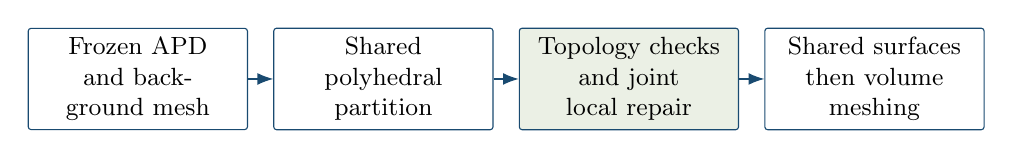
\begin{tikzpicture}[node distance=.32cm, every node/.style={font=\small},
      stage/.style={draw=rubblue,rounded corners=1pt,align=center,minimum height=.85cm,text width=2.55cm},
      arrow/.style={-{Latex[length=2mm]},rubblue}]
    \node[stage] (apd) {Frozen APD\\and background mesh};
    \node[stage,right=of apd] (part) {Shared polyhedral\\partition};
    \node[stage,right=of part,fill=grainA!14] (repair) {Topology checks\\and joint local repair};
    \node[stage,right=of repair] (surf) {Shared surfaces\\then volume meshing};
    \draw[arrow] (apd)--(part);
    \draw[arrow] (part)--(repair);
    \draw[arrow] (repair)--(surf);
  \end{tikzpicture}
  \vspace{.25cm}
  \begin{tabular}{@{}P{.34\textwidth}P{.59\textwidth}@{}}
    \toprule
    Already available & Work proposed here\\
    \midrule
    APD costs, volume fitting & Freeze the source and report complete local topology\\[.13cm]
    Shared polyhedral partition & Modify ownership in a bounded defect neighbourhood\\[.13cm]
    Lloyd conditioning & Compare it as a baseline; add explicit topology acceptance\\[.13cm]
    Surface regularization and Gmsh & Recheck repaired geometry; evaluate FE volume meshing separately\\
    \bottomrule
  \end{tabular}
  \source{Code: power\_diagram.py, apd\_mesh.py, geometry\_conditioning.py, surface\_regularization.py, gmsh\_remeshing.py. Current Gmsh integration generates surface triangles.}
\end{frame}

\begin{frame}{Repairing one grain can disconnect its neighbour}
  \begin{columns}[T,onlytextwidth]
    \begin{column}{.48\textwidth}\centering
      \panel{local_before.png}{3.75cm}\\[-.12cm]
      \textbf{Original partition}\\
      {\small \A{} has a point contact; \B{} is connected}
    \end{column}
    \begin{column}{.48\textwidth}\centering
      \panel{local_greedy.png}{3.75cm}\\[-.12cm]
      \textbf{Candidate: widen only \A}\\
      {\small \A{} is joined; \B{} is disconnected}
    \end{column}
  \end{columns}
  \vspace{.18cm}
  This candidate removes the point defect but must be rejected: grain \B\ loses its connection.
  \source{Constructed $11^3$ voxel partition rendered with Kanapy. Surrounding grain C is hidden in the views but included in every check. Component counts use shared-face adjacency.}
\end{frame}

\begin{frame}{A joint candidate reconnects A and preserves B}
  \begin{columns}[T,onlytextwidth]
    \begin{column}{.43\textwidth}\centering
      \panel{local_joint.png}{4.35cm}\\[-.12cm]
      {\small Widen \A{} and reroute \B}
    \end{column}
    \begin{column}{.53\textwidth}
      \textbf{Measured on this constructed example}
      \vspace{.15cm}
      {\small\setlength{\tabcolsep}{3pt}
      \begin{tabular}{@{}lrrr@{}}
        \toprule
        Grain & A & B & C\\
        \midrule
        Face components & 1 & 1 & 1\\
        Defect voxels & 0 & 0 & 0\\
        Volume change & $+4.69\%$ & $+4.44\%$ & $-0.69\%$\\
        \bottomrule
      \end{tabular}}\par
      \vspace{.25cm}
      Ten of 1331 voxels change ownership. Every voxel still has exactly one grain label.
      \vspace{.25cm}
      \textbf{This demonstrates a joint edit.} Automatic search and admissible volume and shape budgets remain to be developed.
    \end{column}
  \end{columns}
  \source{Kanapy's exhaustive local voxel boundary test reports zero defect-incident voxels for all three grains. This is a discrete example, not a continuous APD repair or an FE result.}
\end{frame}

\begin{frame}{Generate candidates inside a bounded neighbourhood}
  \begin{columns}[T,onlytextwidth]
    \begin{column}{.43\textwidth}\centering
      \panel{local_band.png}{4.4cm}\\[-.1cm]
      {\small Dotted box: editable neighbourhood\\Blue points: protected core locations}
    \end{column}
    \begin{column}{.53\textwidth}
      \begin{enumerate}
        \item Collect cells incident to the defect, plus a halo.
        \item Freeze labels outside the patch and selected grain cores.
        \item Try a finite-width neck and joint neighbour adjustments.
        \item If appropriate, try reassigning a small expendable fragment.
        \item Validate every affected grain. Refine or grow the patch within a fixed budget; otherwise report unresolved.
      \end{enumerate}
    \end{column}
  \end{columns}
  \source{Proposal: use existing clipped APD polyhedra as initial cells. Conforming subdivision may be needed. The candidate search is bounded; it does not guarantee that an admissible repair exists.}
\end{frame}

\begin{frame}{Choose the smallest admissible ownership change}
  \begin{columns}[T,onlytextwidth]
    \begin{column}{.48\textwidth}
      Cell $a$ has volume $|a|$ and label $g$:
      \[
        z_{ag}\in\{0,1\},\qquad \sum_g z_{ag}=1.
      \]
      \[
        V_g=\sum_a |a|z_{ag}.
      \]
      Rank candidates by changed volume and disagreement with the frozen APD costs.
      \vspace{.18cm}
      \textbf{First implementation:} deterministic candidate generation with strict acceptance checks.
    \end{column}
    \begin{column}{.48\textwidth}
      \textbf{Hard acceptance checks}
      \begin{itemize}
        \item Valid boundary links and grain connectivity.
        \item Fixed exterior labels and protected cores.
        \item Cumulative volume bounds and consistent periodic copies.
        \item Required neck size and geometric modification bounds.
      \end{itemize}
      \vspace{.12cm}
      A low objective value cannot override these checks.
    \end{column}
  \end{columns}
  \source{Ownership constraints prevent gaps and overlaps on a valid conforming cell complex. Manifoldness and connectivity require separate checks; this is not an ordinary unconstrained graph-cut problem.}
\end{frame}

\begin{frame}{The difficult tradeoff: topology versus morphology}
  \begin{columns}[T,onlytextwidth]
    \begin{column}{.31\textwidth}\centering
      \panel{neck_surface.png}{3.65cm}\\[-.15cm]
      {\small A finite neck changes the grain geometry}
    \end{column}
    \begin{column}{.65\textwidth}
      \begin{tabular}{@{}P{.35\linewidth}P{.60\linewidth}@{}}
        \toprule
        Requirement & What must be measured\\
        \midrule
        Volume fidelity & Per-grain volume bounds accumulated from the frozen baseline\\[.14cm]
        Shape fidelity & Centroid, covariance, aspect ratio and boundary displacement\\[.14cm]
        Local structure & Neighbour changes, interface areas and junction motion\\[.14cm]
        Resolvable neck & Cross-section relative to the intended FE mesh size\\
        \bottomrule
      \end{tabular}
      \vspace{.2cm}
      A small global volume change can still alter a local load path. Mechanical sensitivity must be tested.
    \end{column}
  \end{columns}
  \source{The illustrated neck is an APD weight control and moves the whole interface. It is not a completed local repair. Tolerances must be chosen for the intended simulation.}
\end{frame}

\begin{frame}{Periodic grains must be checked across opposite box faces}
  \begin{columns}[T,onlytextwidth]
    \begin{column}{.58\textwidth}\centering
      \panel{periodic_slice.png}{3.8cm}\\
      {\small Kanapy periodic APD slice: the two green fragments belong to the same grain}
    \end{column}
    \begin{column}{.38\textwidth}
      \begin{itemize}
        \item Identify opposite faces before counting grain components or boundary links.
        \item Synchronize edits and shared geometry in all corresponding periodic copies.
        \item Do not treat a box cut as a physical grain boundary.
      \end{itemize}
    \end{column}
  \end{columns}
  \source{Constructed two-grain periodic APD evaluated directly by Kanapy. Start the repair prototype with interior, nonperiodic defects; periodic cases are a separate acceptance stage.}
\end{frame}

\begin{frame}{One repaired partition must feed every downstream representation}
  \begin{columns}[T,onlytextwidth]
    \begin{column}{.36\textwidth}\centering
      \panel{pipeline_surface.png}{4.25cm}\\[-.12cm]
      {\small Shared triangles from the current Kanapy geometry builder}
    \end{column}
    \begin{column}{.60\textwidth}
      \begin{enumerate}
        \item Store the repaired labels and cell complex as the authoritative geometry.
        \item Extract each interface once from neighbouring cells with different labels.
        \item Regularize and remesh surfaces, then repeat topology and intersection checks.
        \item Evaluate a conforming volume mesher and check element quality, grain labels and periodic matching.
      \end{enumerate}
      \vspace{.15cm}
      Reapplying the original APD minimum inside the repaired patch would undo the repair.
    \end{column}
  \end{columns}
  \source{Current Kanapy output is a surface mesh. Planned volume-meshing comparators: CGAL Mesh\_3 and XtalMesh.}
\end{frame}

\begin{frame}{Test against known defects and complex RVEs}
  \small
  \begin{tabular}{@{}P{.28\textwidth}P{.29\textwidth}P{.35\textwidth}@{}}
    \toprule
    Cases & Comparisons & Recorded outcomes\\
    \midrule
    Point and edge contacts; normal junction controls & Current pipeline; existing conditioning; local repair & Defects removed, new defects, unresolved cases\\[.12cm]
    Fixed packed APDs at several resolutions & Freeze centres, matrices and weights; refine background & Approximation error separated from repair changes\\[.12cm]
    Complex and periodic RVEs & Repeated seeds and paired geometry & Per-grain volume, moments, adjacency and runtime\\[.12cm]
    Meshed repaired partitions & Identical loading and material assignment & Positive Jacobians, mesh convergence, elastic response and local stress\\
    \bottomrule
  \end{tabular}\par
  \normalsize
  \vspace{.28cm}
  \textbf{First deliverable:} a complete combinatorial report for the reconstructed partition and a bounded repair prototype. Validation on Hartmaier's case needs its saved input.
  \source{The benchmark will record unresolved cases, geometric changes, downstream mesh quality and mechanical sensitivity.}
\end{frame}

\begin{frame}{Proposed implementation order}
  \begin{columns}[T,onlytextwidth]
    \begin{column}{.62\textwidth}
      \begin{enumerate}
        \item Complete the per-grain topology report and save failing inputs.
        \item Implement the smallest interior repair patch with full neighbour checks.
        \item Add volume and morphology budgets, refinement and rejection logic.
        \item Extend to periodic defects; rebuild shared surfaces.
        \item Benchmark volume meshing and mechanical sensitivity.
      \end{enumerate}
      \vspace{.2cm}
      Each stage should return a saved geometry and a report that can be inspected.
    \end{column}
    \begin{column}{.33\textwidth}\centering
      \panel{local_joint.png}{3.05cm}\\[-.1cm]
      {\small Constructed joint edit}
      \vspace{.2cm}
      \raggedright
      \textbf{Decisions to agree:} allowable volume and shape changes, treatment of small fragments, and target FE mesh scale.
    \end{column}
  \end{columns}
\end{frame}

\appendix

\begin{frame}[noframenumbering]{Backup: the analytical APD control}
  \begin{columns}[T,onlytextwidth]
    \begin{column}{.32\textwidth}\centering
      \panel{split_surface.png}{2.55cm}\\[-.1cm]
      {\small $\Delta w<0$: separated lobes}
    \end{column}
    \begin{column}{.32\textwidth}\centering
      \panel{pinch_surface.png}{2.55cm}\\[-.1cm]
      {\small $\Delta w=0$: point contact}
    \end{column}
    \begin{column}{.32\textwidth}\centering
      \panel{neck_surface.png}{2.55cm}\\[-.1cm]
      {\small $\Delta w>0$: finite neck}
    \end{column}
  \end{columns}
  \[
    q_i(\mathbf{x})=(\mathbf{x}-\mathbf{c}_i)^T A_i(\mathbf{x}-\mathbf{c}_i)-w_i,
    \quad g(\mathbf{x})=\arg\min_i q_i(\mathbf{x}).
  \]
  With coincident centres $(.5,.5,.5)$, $A_1=I$, $A_2=\mathrm{diag}(2,2,.5)$:
  \[
    \overline{\Omega_2}=\{\mathbf{x}:
    (x-.5)^2+(y-.5)^2-\tfrac12(z-.5)^2\leq\Delta w\}.
  \]
  \source{Existing regression: test\_power\_diagram\_diagnostics.py. Surface geometry uses the grain closure; pointwise ties go to the first grain. These deliberately coincident seeds are a control, not packed particles.}
\end{frame}

\begin{frame}[noframenumbering]{Backup: candidate ranking and rejection}
  \small
  For atomic cells $a$ in the patch, propose:
  \[
    E(z)=\alpha\sum_a |a|\,[g_a\ne g_a^0]
       +\beta\sum_a\int_a\bigl(\widetilde q_{g_a}(\mathbf{x})
                          -\min_j\widetilde q_j(\mathbf{x})\bigr)\,d\mathbf{x}.
  \]
  \begin{itemize}
    \item Freeze piecewise-affine costs $\widetilde q$ and retain original clipped-atom boundaries during refinement.
    \item Integrate affine cost differences using atom volumes and centroids; normalize objective terms.
    \item Enforce volume bands $|V_g-V_g^0|\leq\delta_g$; exact equality may be infeasible with fixed atoms.
    \item Enforce connectivity, boundary links, neck size and protected cells separately.
    \item Bound refinement and patch expansion; report unresolved if no candidate passes.
  \end{itemize}
  \source{The objective is proposed. A finite candidate search guarantees termination or rejection, not a feasible repair or a global optimum. Geometric subdivision must remain conforming across patch boundaries.}
\end{frame}

\begin{frame}[noframenumbering]{Backup: why BFS is only one part of validation}
  \begin{columns}[T,onlytextwidth]
    \begin{column}{.44\textwidth}\centering
      \panel{local_greedy.png}{3.5cm}\\[-.1cm]
      {\small All voxel boundary links pass here, but grain B has two volume components}
    \end{column}
    \begin{column}{.52\textwidth}
      \textbf{Three separate questions}
      \begin{enumerate}
        \item Connected volume? Use BFS on shared faces.
        \item Valid local surface? Check edges and vertex links.
        \item Usable FE geometry? Check intersections, feature size and mesh quality.
      \end{enumerate}
      \vspace{.16cm}
      A connected grain can still have a local self contact. Multiple boundary shells may also describe a valid cavity.
    \end{column}
  \end{columns}
  \source{The existing EBSD graph is a separate 2D workflow. Its pixel connectivity does not certify a 3D grain hull. Periodic volume components must be counted after face identification.}
\end{frame}

\begin{frame}[noframenumbering]{Backup: a concrete first candidate generator}
  \begin{columns}[T,onlytextwidth]
    \begin{column}{.35\textwidth}\centering
      \panel{local_band.png}{3.3cm}\\
      {\small Adjacency follows shared cell faces}
    \end{column}
    \begin{column}{.61\textwidth}\small
      \begin{enumerate}
        \item Locate the defective grain sectors.
        \item Generate $K$ candidate cell paths, ranked by changed volume and APD cost.
        \item Expand paths to the required neck cross-section.
        \item Branch over donor rerouting or another target-grain path.
        \item Limit joint edits to $D$; validate every complete candidate.
      \end{enumerate}
      \vspace{.1cm}
      Contract exterior components to fixed terminals and preserve their connections.
    \end{column}
  \end{columns}
  \source{Proposed candidate generator, not implemented. Paths do not certify topology. Limit search, patch growth and refinement; report unresolved if none passes.}
\end{frame}

\begin{frame}[noframenumbering]{Backup: repository sources}
  \small
  \textbf{Repository sources}
  \begin{itemize}
    \item \code{examples/RVE\_generation/create\_rve.py}: adapted packing and voxel workflow.
    \item \code{tests/test\_power\_diagram\_diagnostics.py}: controlled APD pinch.
    \item \code{tests/test\_apd\_boundary.py}: ordinary junction control.
    \item \code{apd\_geometry.py}, \code{plotting.py}, \code{voxelization.py}: surfaces, images and voxel checks.
    \item \code{geometry\_conditioning.py}, \code{surface\_regularization.py}: existing baselines.
  \end{itemize}
  \vspace{.2cm}
  \normalsize
  Every grain image uses Kanapy labels or Kanapy surface triangles. Source geometries, parameters and measurements are saved with the figure script.
  \source{The old PyVista example uses an obsolete global vertex key. Figures use the current APD data structures and Matplotlib. The contextual RVE is illustrative; no actual failing specimen from Hartmaier was available.}
\end{frame}

\begin{frame}[noframenumbering]{Backup: literature and downstream meshing}
  \small
  \begin{itemize}
    \item \href{https://doi.org/10.1016/j.commatsci.2024.113317}{Buze et al. (2024), Computational Materials Science 245, 113317}: APDs and generalized Lloyd conditioning; empirical improvement is not a topology theorem.
    \item \href{https://doi.org/10.1016/j.proeng.2015.10.132}{Zhang, Cha and Bajaj (2015), Procedia Engineering 124, 187--199}: repair material classification before extracting shared surfaces.
    \item \href{https://doi.org/10.1007/s40192-022-00251-w}{Hestroffer and Beyerlein (2022), XtalMesh}: comparator for polycrystal volume meshing.
    \item \href{https://doc.cgal.org/latest/Mesh_3/group__PkgMesh3Functions.html}{CGAL Mesh\_3 documentation}: volume meshing options do not repair invalid input topology.
  \end{itemize}
  \vspace{.2cm}
  These sources support the architecture and provide comparators. They do not establish the proposed repair's robustness or preservation of microstructural statistics.
\end{frame}

\end{document}
